%!TEX TS-program = xelatex
%!TEX encoding = UTF-8 Unicode
%!TEX root = 2024-gs-adonis-template.tex
%
\documentclass{gs-adonis}
\usepackage[english,italian]{babel}
%-------------------------------------------------------------------------------
%--------------------------------------------------------------------- CUSTOMS -
%-------------------------------------------------------------------------------
% \usepackage{showframe}
% \renewcommand\ShowFrameLinethickness{0.15pt}
% \renewcommand*\ShowFrameColor{\color{red}}
% %
% \usepackage{tikz}
% \usetikzlibrary{
%   shapes,
%   through,
%   calc,
%   intersections,
%   backgrounds,
%   positioning,
%   decorations.text
%   }
% \usetikzlibrary{arrows.meta}
% \usetikzlibrary{bending}
\usepackage[
  small,
  labelfont=bf,
  up,
  textfont=it,
  up
  ]{caption}
%
\usepackage{paralist}
\usepackage{subfigure}
%\usepackage{glossaries}
%\input{includes/glossario.tex}
%\makeglossaries
\usepackage{csquotes}
\usepackage[style=ieee,backend=biber]{biblatex}
\bibliography{includes/bibliografia.bib}
\usepackage{enumitem}
\usepackage{adjustbox}
\usepackage{hhline}
\DeclareLabelname[movie]{
    \field{director}
    \field{producer}
  }
\usepackage{scrextend}
\usepackage{calc}
\usepackage{mwe}

\usepackage{todonotes}
\usepackage{hyperref}
%-------------------------------------------------------------------------------
%------------------------------------------------------------------------ MAIN -
%-------------------------------------------------------------------------------
\title{Autocostruzione di un interprete.\\
       Per quale musica?}
\subtitle{Progetto di \emph{Dottorato di Ricerca in Composizione e Performance musicale}}
\author{Alice Cortegiani \textsuperscript{1}}
% secondary details
%\affiliation{\textsuperscript{1} Spherical Technologies SRLS}
\correspondence{alicecortegiani@gmail.com}
\version{\today}
% headers
\runningauthor{Alice Cortegiani}
\runningtitle{Autocostruzione di un interprete. Per quale musica?}
%-------------------------------------------------------------------------------
%--------------------------------------------------------------------- COMANDI -
%-------------------------------------------------------------------------------
% \newcommand{\studi}{\emph{Sei studi di Agamotto sul Tempo}}
% \newcommand{\tempo}{\emph{Tempo}}
% \newcommand{\canto}{\emph{canto alla durata}}
%-------------------------------------------------------------------------------
%-------------------------------------------------------------------- ABSTRACT -
%-------------------------------------------------------------------------------
\abstract{%
  %\begin{addmargin*}[0pt]{-\marginparsep-\marginparwidth}
  \input{includes/abstract.txt}
  %\end{addmargin*}
}
%-------------------------------------------------------------------------------
%-------------------------------------------------------------------- DOCUMENT -
%-------------------------------------------------------------------------------
\begin{document}
\maketitle
%\input{includes/000-citazioni.tex}
%
%\clearpage
%-------------------------------------------------------------------------------
%--------------------------------------------------------------------- APPUNTI -
%-------------------------------------------------------------------------------
% \section*{APPUNTI}
% \begin{compactitem}
%   \item questione etica
%   \item diagrammi a blocchi
%   \item storia di una ricerca, fagioli, sogno, immagine
%   \item rappresentazione
%   \item feedback
%   \item interfaccia
%   \item tecnica
%   \item musica
%   \item invenzione
%   \item{bibliografia da compilare:}
%   \begin{compactitem}
%     \item Bergson
%     \item Barthes
%     \item Borges
%     \item Branchi
%     \item Cacciari
%     \item Candiani
%     \item Di Scipio
%     \item Galante
%     \item Guaccero
%     \item Handke
%     \item Ferraris
%     \item Lupone
%     \item Netti
%     \item Nono
%     \item Ronchi
%     \item Sartre
%   \end{compactitem}
% \end{compactitem}
%
%\clearpage
%-------------------------------------------------------------------------------
%--------------------------------------------------------------------- APPUNTI -
%-------------------------------------------------------------------------------
%\tableofcontents
%\clearpage
%-------------------------------------------------------------------------------
%-------------------------------------------------------------------- INCLUDES -
%-------------------------------------------------------------------------------
% \input{includes/000-introduzione.tex}
% \input{includes/100-ciclobase.tex}
% \input{includes/200-cad.tex}
% \input{includes/300-tempo.tex}

% \clearpage
%
% \tiny
% \twocolumn
% \printglossary[title={glossarietto}]
%
% \clearpage

%\normalsize
%\onecolumn

\section*{keywords}

[massimo 5 key words]


\section{descrizione del progetto di ricerca}% (massimo 2.000 parole / 2.000 words)}

\subsection{descrizione del soggetto di ricerca}% (600 parole):}

%\emph{a) descrivere l’ambito generale e lo stato dell’arte della pratica musicale in cui e attraverso cui si desidera svolgere il proprio progetto;}

La ricerca sul suono, nelle possibilità individuabili attraverso la ricerca
artistica musicale, nell'articolazione delle peculiarità di cui essa dispone,
determina l'ambito generale in cui il progetto si inscrive tracciando percorsi
unici e di indipendenza dalla ricerca scientifica e universitaria. I luoghi
della ricerca, i soggetti coinvolti e gli oggetti individuati sono accessibili
e attivi al solo processo artistico musicale.

L'ambito generale in cui il progetto si inscrive è quello della musica di
ricerca che, con radici profonde nei piccoli laboratori sperimentali sorti nel
novecento, oggi è fortemente rappresentato da centri di ricerca storici e
nuovi laboratori indipendenti, la cui attività si riversa nella pratica, nella
didattica e nella divulgazione musicale a piu livelli.

Nel contesto così descritto, parole come \emph{Suono, Rumore, Timbro},
con indipendenza di indagine da altre discipline, nella ricerca musicale
acquisiscono strumenti unici di esperienza e conoscenza: ascolto, ambiente,
ambiente in ascolto (gli ascoltatori), in un livello di contro-reazione
(feedback) possibile solo in condivisione di un processo musicale.

Il progetto si struttura attraverso le relazioni che intercorrono tra opera,
strumento (il clarinetto) e interprete nel processo creativo di ricerca che
porta alla produzione di nuova musica. Mediante analisi del repertorio che
concede esplorazione radicale dello strumento, analisi dei segnali prodotti
dallo strumento con l'uso di tecnologie in grado di descriverne il
comportamento spaziale (che coincide con quello timbrico), una scrittura
dedicata all'esplorazione (dello strumento e della scrittura stessa) il
clarinetto si definisce a luogo di pensiero ed esplorazione, di esperienza e
consapevolezza, verso un pensiero creativo che possa definirsi in prassi.
%in continua tendenza verso presupposti utopici, in ascolto.

Il progetto si inserisce in una pratica quotidiana di ricerca presso laboratori
e centri specializzati, in una pratica musicale attenta alle necessità di un
pensare creativo e analitico, in cui il ruolo dell'interprete possa rinascere
dalle ceneri dell'intrattenimento cameristico, operistico e sinfonico.

\begin{figure}[ht]
  \centering
  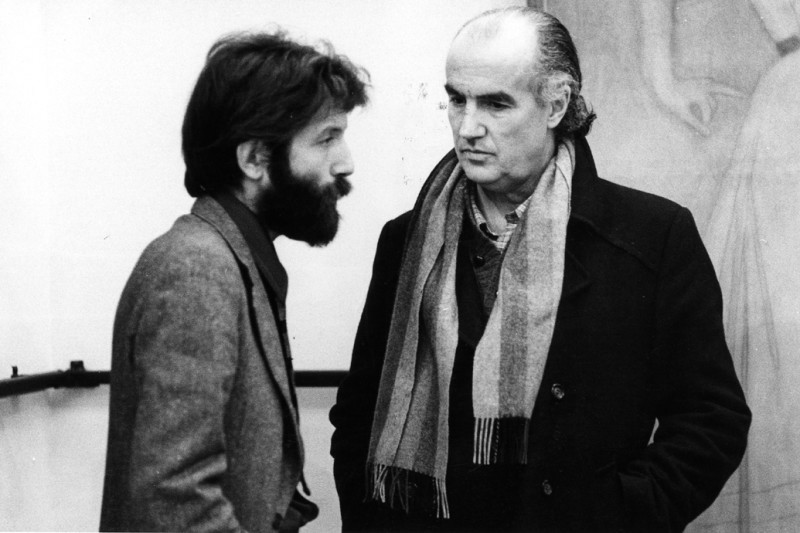
\includegraphics[width=\linewidth]{images/luigi-nono-massimo-cacciari.jpg}
  \captionsetup{width=.81\linewidth}
  \caption{Masimo Cacciari, Luigi Nono.}
  \label{cacciari}
\end{figure}

%\emph{b) formulare il problema e una o più domande di ricerca relative ad esso che possano guidare l’esplorazione dell’argomento.}

% Definizione del problema
% 2. Definizione dell’obiettivo della ricerca
% 3. Scelta del disegno dello studio
% 4. Individuazione delle variabili da studiare
% (scelta e definizione)
% 3. Raccolta dei dati
% 4. Valutazione della qualità del dato
% 5. Elaborazioni statistiche
% 6. Interpretazione dei risultati
% 7. Comunicazione e trasferimento nella pratica
% dei risultati della ricerca
%
% Formulare quesiti generali di ricerca
%  Effettuare indagini bibliografiche mirate sugli
% argomenti connessi con i quesiti
%  Sviluppare uno schema concettuale/teorico di
% inquadramento dei problemi conoscitivi oggetto
% di studio
%  Scegliere gli obiettivi di ricerca

\begin{figure}[ht]
  \centering
  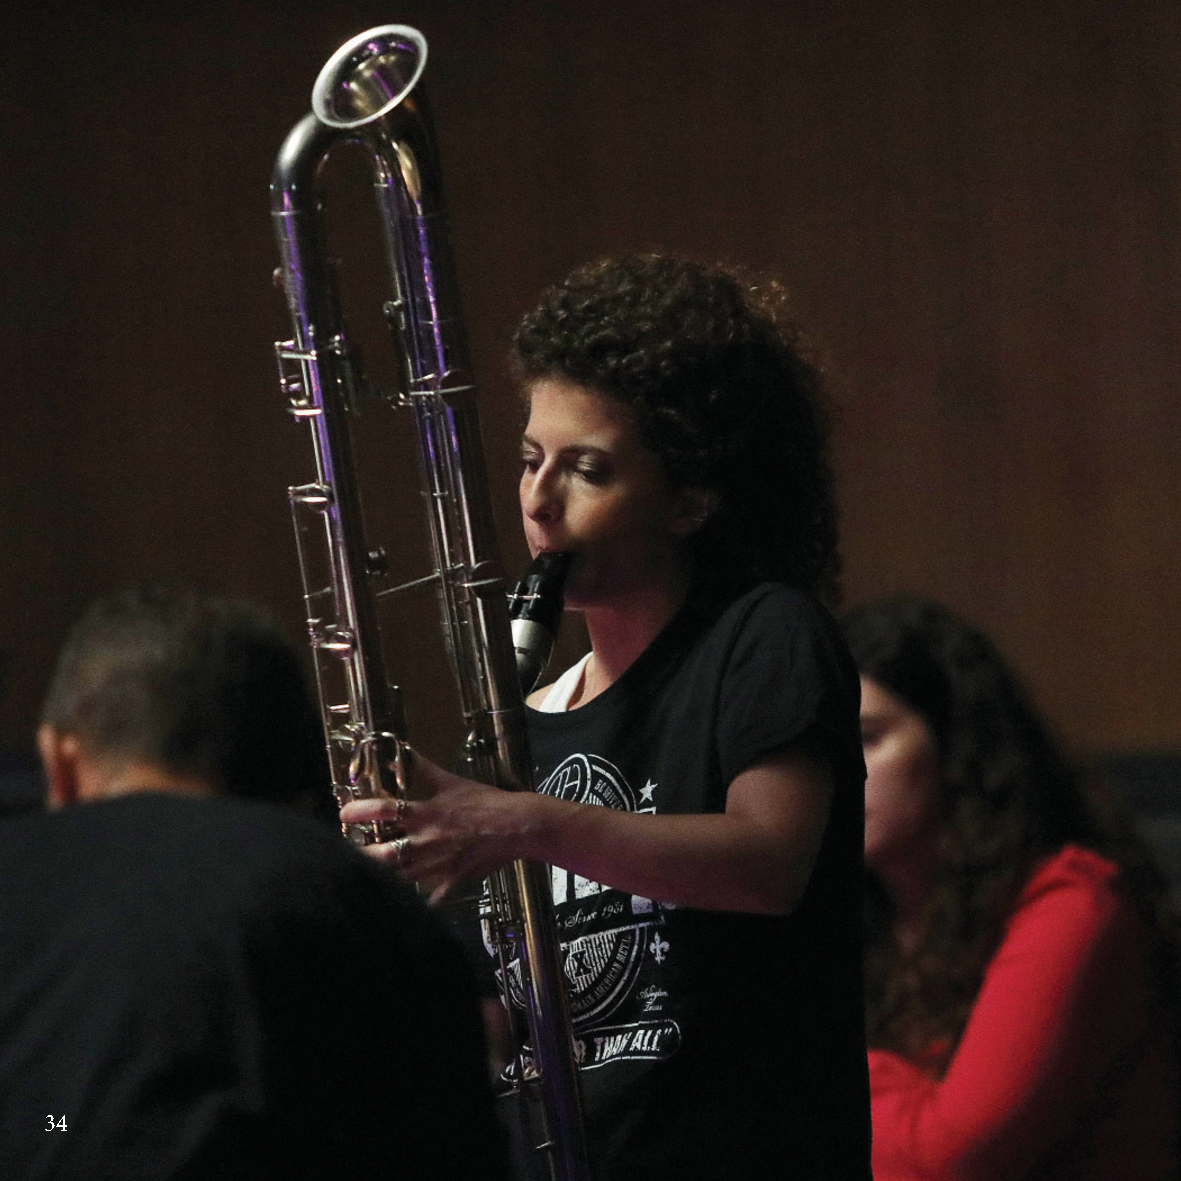
\includegraphics[width=\linewidth]{images/panthera.pdf}
  \captionsetup{width=.81\linewidth}
  \caption{Interprete? o Zebra}
  \label{alice}
\end{figure}

\emph{Che cos'è un interprete?}

Massimo Cacciari nel descrivere il tema dell'ascolto in Luigi Nono
\cite{Cacciari1995} disegna lo sfondo di una problematica filosofica che assale
la cultura occidentale nelle relazioni tra scrittura-voce-ascolto. Problemi di
ordine generale che si riferiscono al significato culturale generale della
nascita della scrittura alfabetica e che in un lento processo vede il dominio
della \emph{visione} sull'\emph{ascolto} in una

\begin{quote}
  progressiva desomatizzazione della voce. Una perdita dell'udire. L'udire
  non è più una funzione fondamentale del comprendersi. \cite{Cacciari1995}
\end{quote}

Egli sottolinea che in molte pratiche artistiche questo problema può essere
dimenticato, può non essere un problema, ma non nella musica: la musica non può
essere senza ascolto. La perdita della memoria, dell'ascolto, della memoria
dell'ascolto è fatale per la musica. Questo accade perché ad ogni ascolto muta
il testo stesso. La musica non può esistere senza un ascolto vivente, attivo.

In questo quadro di sensibilità musicale, l'interprete per primo, cercando di
comprendere, di capire che vorrebbe riuscire a comprendere di più ciò che c'è
\emph{prima del primo suono e dopo l'ultimo suono} \cite{Cacciari1995}, si fa
testimone della ricerca musicale nel luogo sonoro in cui opera in grado di
\emph{articolare, accentuare, dare al canto}, il testo musicale: a chiarire
anche la distanza dall'esecutore \emph{l'interprete non legge} il testo
musicale, \emph{lo riattiva, lo da al canto} \cite{Cacciari1995}.

\emph{Che cos'è il repertorio?}

Intraprendere il percorso di interprete della musica contemporanea di ricerca è
un atto che conduce inevitabilmente all'individuazione di problemi nel campo
della formazione accademica. Questa, incentrata sullo studio del repertorio
classico, attraverso gli esiti della de/formazione, confonde il ruolo
dell'esecutore con la figura dell'interprete, consumato nel fine prestabilito
dal dominio dell'intrattenimento, cristallizzando la sensibilità del musicista
in una prassi parziale, ma resa assoluta, quindi distorta e precludendo così
fondamentali contributi nel campo della ricerca musicale, di un fare musicale
condiviso e contemporaneo.

% I programmi di studio dei corsi strumentali adottati dai conservatori di musica
% italiani favoriscono un percorso formativo fondato sul repertorio d'intrattenimento,

% La prassi del repertorio di musica
% contemporanea di ricerca costruisce e si costruisce attraverso lo strumento
% come strumento di pensiero, l'interprete è anello attivo della catena, generato
% e generatore.
%
% con conseguente esito di edificazione del musicista attraverso una parziale e distorta prassi, che rende totalizzante la visione limitata, ridotta.

% I programmi di studio dei corsi strumentali adottati dai conservatori di musica italiani favoriscono un percorso formativo
% fondato sul repertorio d'intrattenimento, cristallizzando la sensibilità del musicista in una prassi parziale resa assoluta,
% quindi distorta.
% Riconoscere la pluralità del repertorio è elemento essenziale per avere accesso, dalla teoria,
% alla complessità dei linguaggi musicali strutturati.
% La prassi del repertorio di musica contemporanea di ricerca costruisce e si costituisce nel processo;
% attraverso lo strumento acustico, strumento di pensiero, l'interprete è anello attivo della catena, generato e generatore.
%
% Nel dominio dell'intrattenimento la chiave di lettura tende, sovente, erroneamente a sottovalutare aspetti fondamentali di apporto storico-sociale
% che hanno nutrito la creazione musicale, favorendo ambizione e gratificazione nel risultato alla riproduzione del testo scritto.
% Reperire, trovare, partecipare al processo creativo di musica contemporanea di ricerca comporta un costante confronto:
% con le domande fondamentali di cui si nutre la prassi interpretativa, con gli strumenti da costruire per avere accesso al dialogo con
% interlocutori dediti ad pensiero in ascolto, volti alla creazione e quindi nel reperire opere di ricerca dal pensiero musicale.

\emph{Che cos'è contemporaneo?}

\begin{quote}
  Contemporaneo è colui che riceve in pieno viso il fascio di tenebra che proviene dal suo tempo. \cite{agamben2008che}
\end{quote}

La contemporaneità è quindi un momento mobile del tempo che identifica la
facoltà di osservare l’oscurità del tempo specifico, quella relazione col
tempo che aderisce a esso attraverso una sfasatura e un anacronismo che ci
permette di valutare, vedere ed analizzare, alla dovuta distanza. Distanza da
cosa?

Fare repertorio contemporaneo, nella contemporaneità, nell’espressione del suo
senso più completo è imparare ad ascoltare: \emph{Suono, Rumore, Timbro} e Silenzio.

\emph{Che cos'è la ricerca musicale contemporanea e come può formarsi l'interprete contemporaneo?}

\subsection{Metodi e processo di ricerca}% (600 parole):}

%\emph{a) descrivere cosa si intende fare in termini pratici per indagare il proprio argomento di ricerca;}
%Il percorso di ricerca parte dall'analisi musicale di luz (già avviata con quattro interpretazioni in concerto)
%e giunge alla catalogazione sistematica delle possibilità timbriche del clarinetto
%contrabbasso nelle due tipologie (metallo e legno) sotto la guida di …
\begin{description}
  \item[Analisi:] Domenico Guaccero, \emph{Luz (da Descrizione del corpo) per strumento grave}.
  Guaccero, dalla sua vocazione alla ricerca artistica musicale, ha osservato con vivacità
  ed acutezza plurime tessiture del vivere la contemporaneità, sempre alimentata
  dalla necessità di dare corpo nel fare musicale e nell'azione sociale.
  \emph{Luz}, dalle emersioni del corpus di opere, si pone in continuità con
  il Contemporaneo in quanto illumina dal fascio di tenebre da cui è forgiata.

  Melodie di \emph{Timbro} articolato in 24 differenti tipologie, Silenzio
  \emph{udibile animato} e Grafia musicale, fondono nucleo centrale della spirale
  di speculazioni di esperienza e conoscenza.
  Gli strumenti coinvolti alla messa in ascolto:

  Clarinetto Contrabbasso

  TETRAREC

  STONE

  LUz lamps

  L'opera ha dato impulso al progetto di ricerca.
  Dal gennaio del 2023 è stata ascoltata in quattro interpretazioni in concerto,
  complementari alle indagini di laboratorio.
  Allo stato attuale giunge alla catalogazione sistematica delle possibilità
  timbriche del clarinetto contrabbasso nelle due tipologie, metallo e legno
  attraverso tecnologie e strumenti di ascolto [\ldots] TETRAREC %<3
\end{description}

\begin{description}
  \item[Percorso di approfondimento con Giorgio Netti: \emph{Che cos'è uno strumento?}]
  Il clarinetto contrabbasso, strumento-luogo periferico.
  Scrittura di esplorazione, dello strumento e della scrittura stessa.
  \begin{quote}
  Chi  ha  esperienza  nel  campo  dell’esplorazione  (non  specificatamente
  strumentale) sa che molto spesso la quantità d’informazione relativa ad un
  argomento  è  talmente  ricca  da  diventare  essa  stessa  un  problema.
  Dove tutto  è differentemente  importante  nulla  è  più  importante  e  si
  rimane abbandonati sulla riva senza saper che fare: dunque, farsi ammaliare dal
  suono-sirena si ma, prendendo esempio da Ulisse, nume tutelare di tutti gli
  esploratori, farsi ammaliare legati\ldots
  \end{quote}
    Esplorando il clarinetto contrabbasso, luogo di pensiero, in maniera radicale,
    sferica, è subentrata la necessità di estendere la pratica corporea ad una
    conoscenza più stratificata, approfondita e lontana dai filtri di quanto ad oggi
    risulta evinto. Un percorso con l'intento di contestualizzare, integrare e superare
    l’interpretazione abituale dei vari elementi caratterizzanti dello strumento.
    Con la guida della profonda attenzione di Netti nella tendenza ad
  \begin{quote}
    esplorare gli strumenti come se fossero città antiche: ognuno di loro con un
    suo centro storico costituito da tutto ciò a cui scolasticamente associamo a
    quello strumento ed una periferia, progressivamente meno definita, fatta da
    ciò che è incerto, meno omogeneo, nascosto.
  \end{quote}
  Esplorare, in maniera inalterata un luogo, originale. Porlo in relazione dalla
  prospettiva da cui non è stato ascoltato, predisporre zone periferiche dello stesso
  per una prima mappatura che tracci come quelle particolarità, caratteristiche,
  o meglio
    \begin{quote}
      criticità, si relazionino all'intera storia dello strumento o piuttosto
      come è ascoltata o pensata a partire da quella caratteristica, l'intera
      storia dello strumento assume una prospettiva differente che in dialogo con
      le precedenti contribuisce ad estenderne i confini, e quindi, il senso._
  \end{quote}

  verso l'organizzazione di un \emph{Catalogo} che emerga dall' \emph{andare incontro} allo strumento.
\end{description}

\begin{description}
  \item[Catalogo - Co.Si.]
\end{description}

\begin{description}
  \item[ccb tempo]
\end{description}

\begin{description}
  \item[Lupone]
\end{description}


%Opera originale Lupone (con elettronica)

%Opera con strumenti d'invenzione SILVI %<3


\begin{figure}[ht]
  \centering
  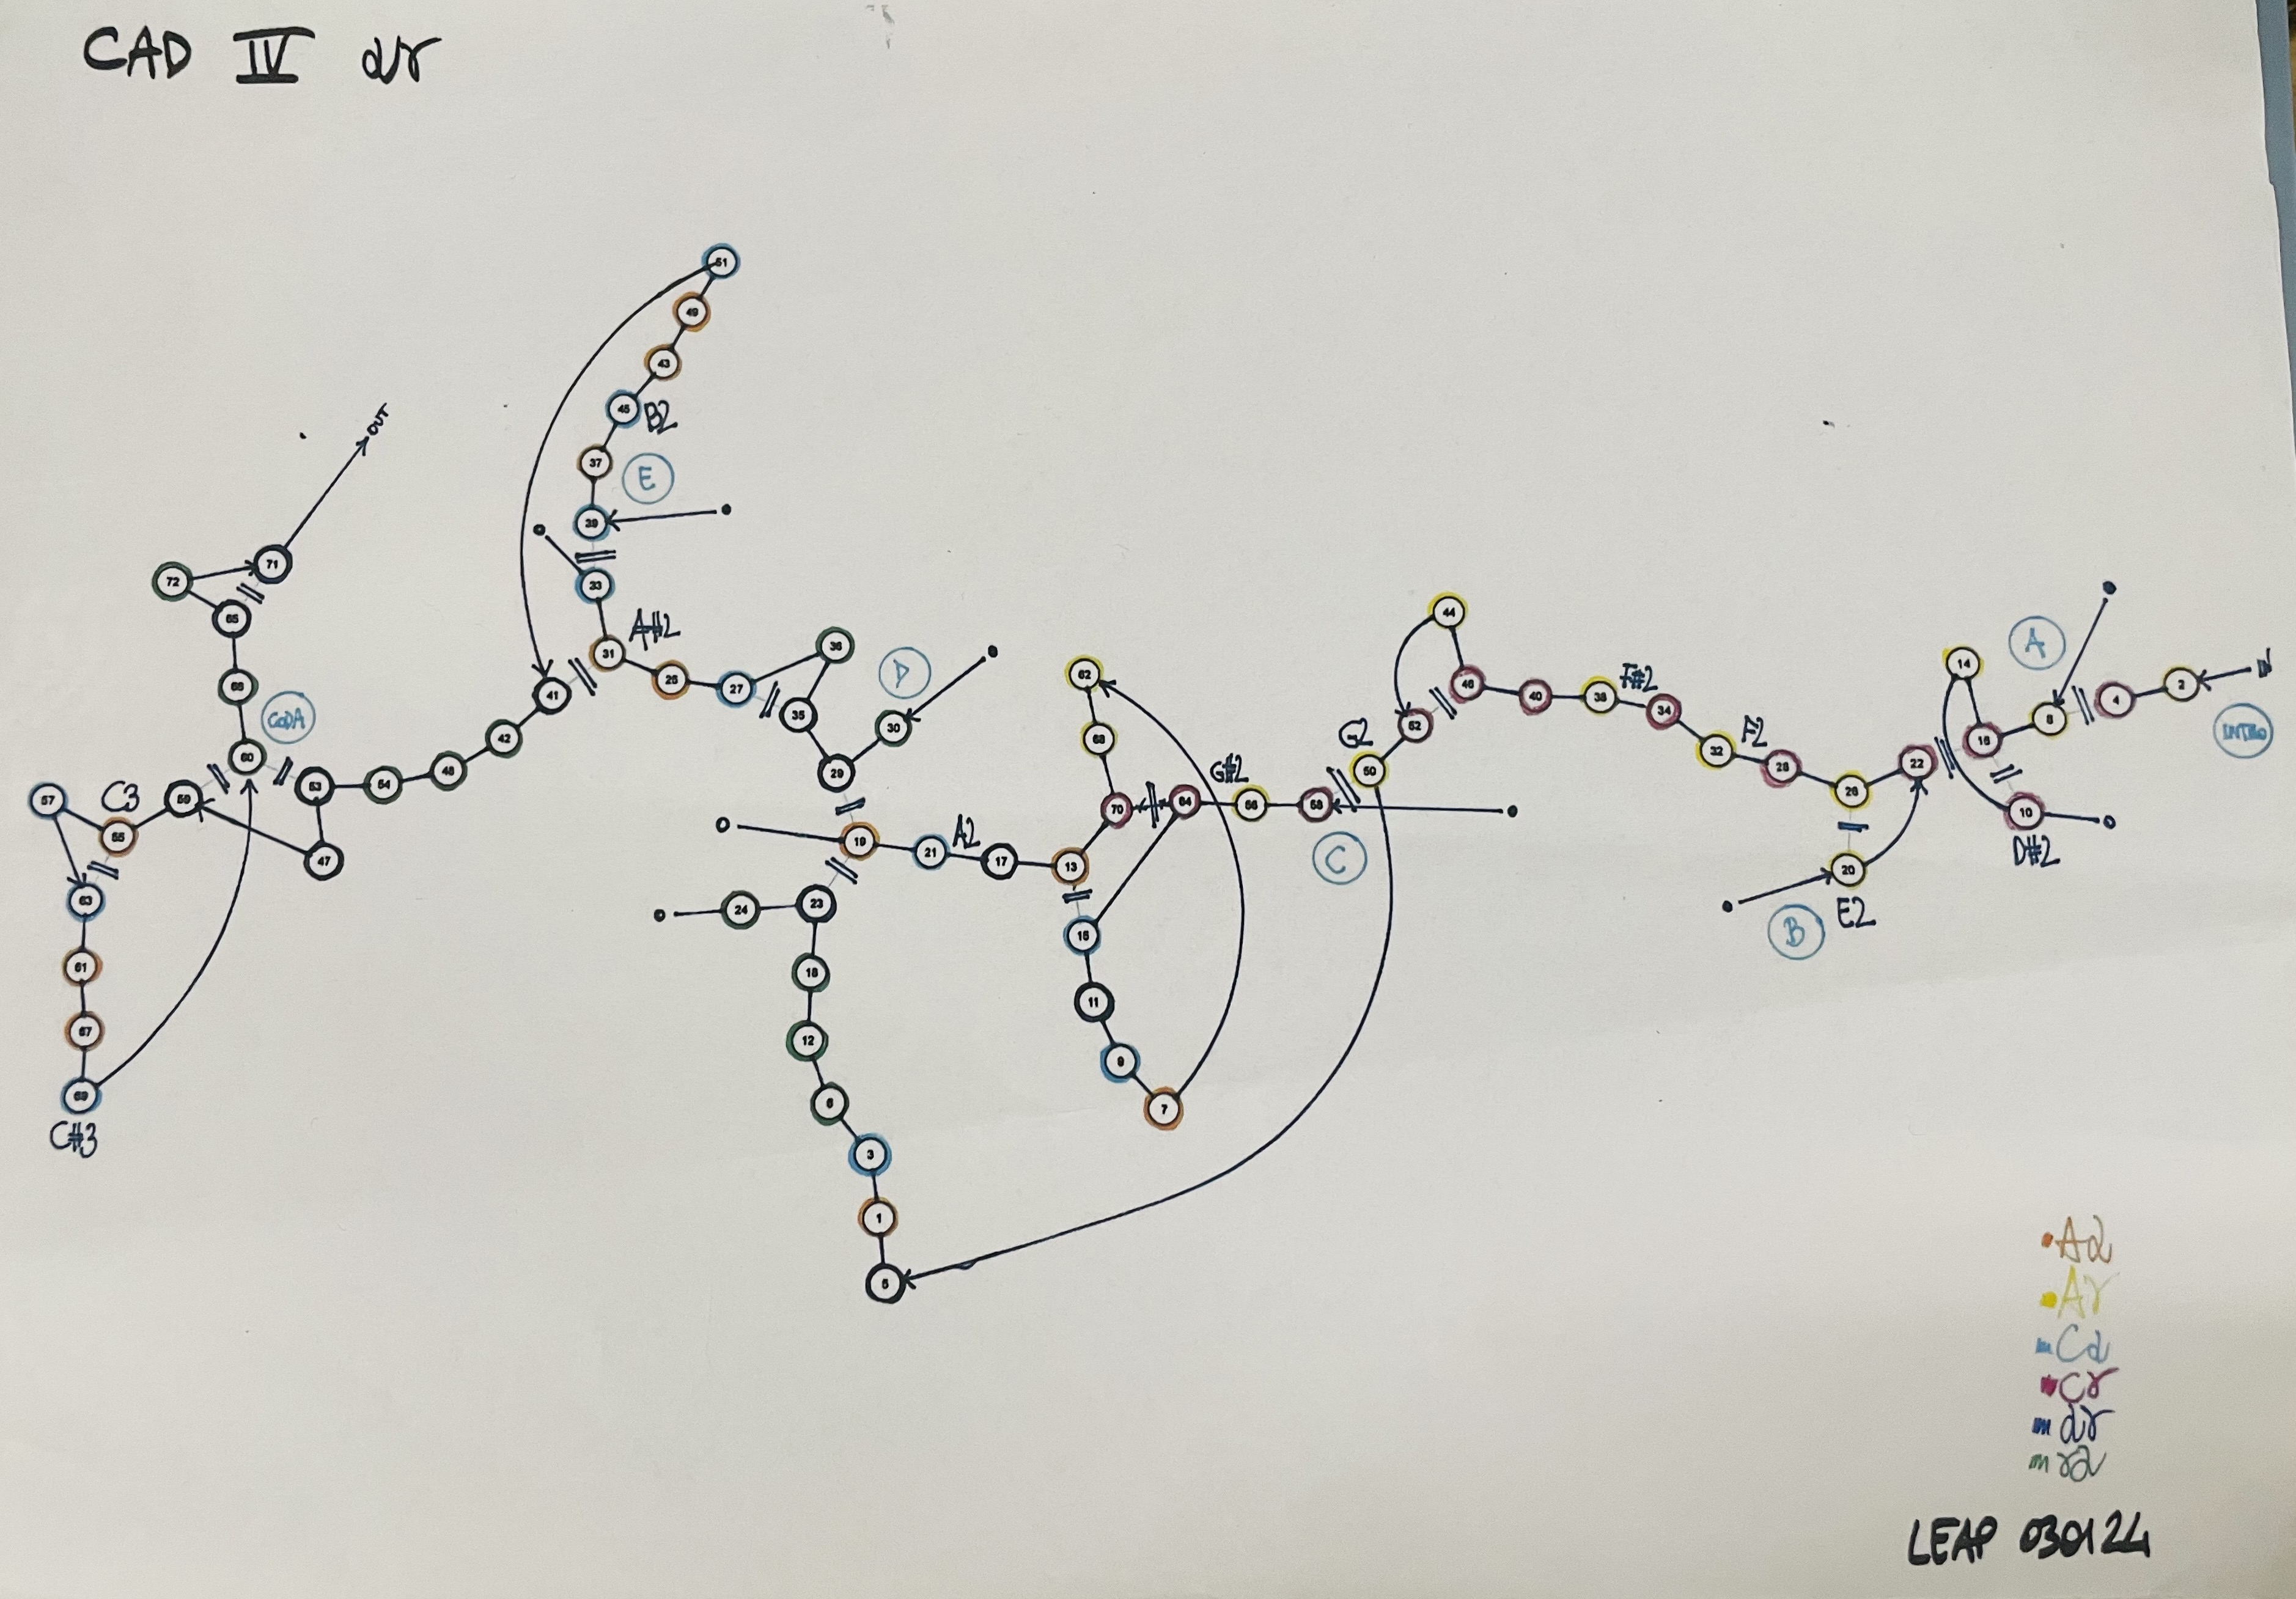
\includegraphics[width=\linewidth]{images/cad-IV-grafo.jpg}
  \captionsetup{width=.81\linewidth}
  \caption{Grafo}
  \label{grafo}
\end{figure}

\begin{figure}[ht]
  \centering
  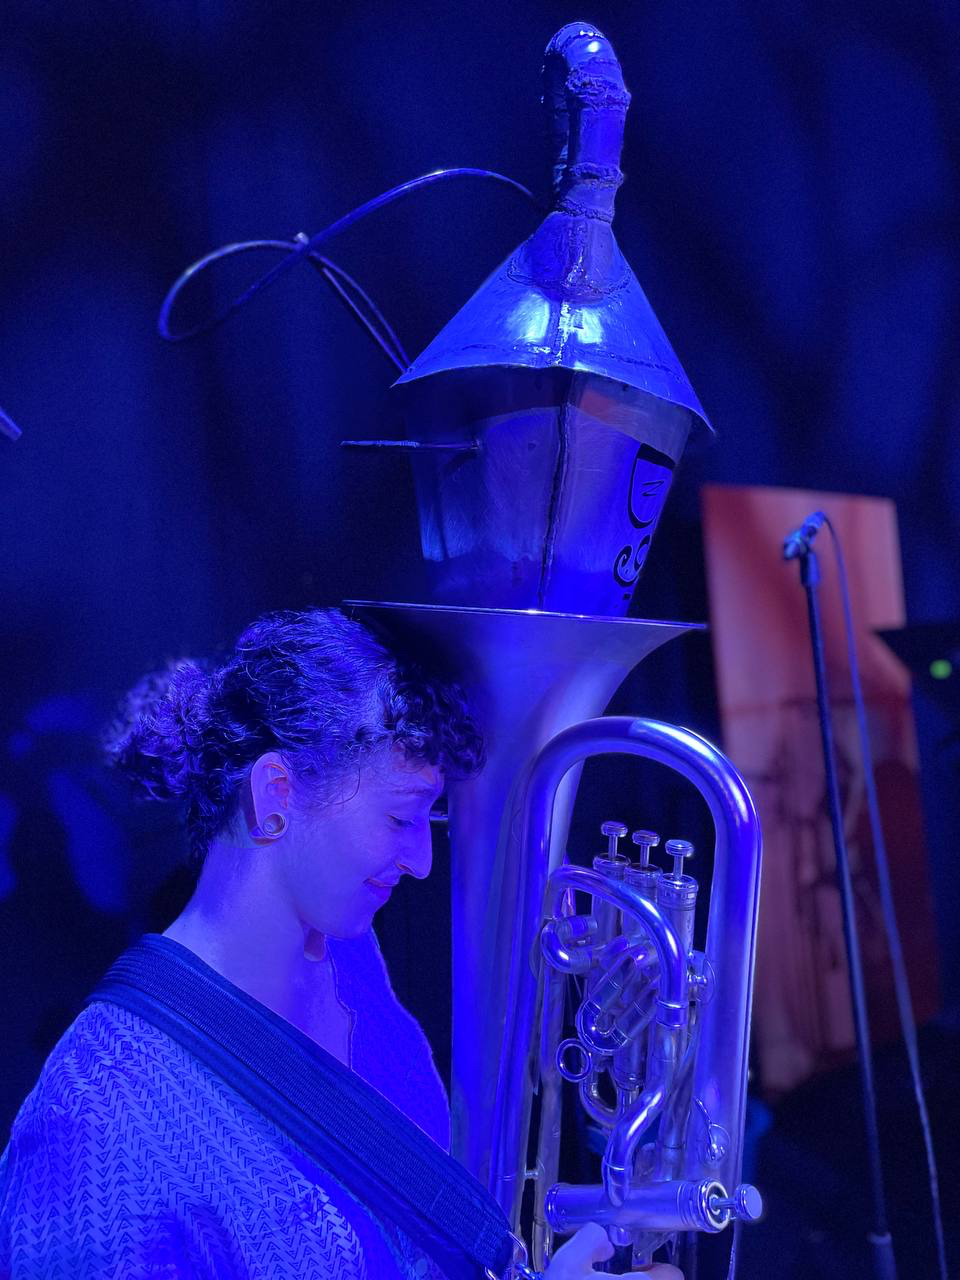
\includegraphics[width=\linewidth]{images/IMG_F5A47D566D6E-31.jpeg}
  \captionsetup{width=.81\linewidth}
  \caption{Sistema Bo.Si.}
  \label{bosi}
\end{figure}

Estero?

% identificare un problema di ricerca
%  esplicitare e chiarire gli obiettivi
%  disegno della ricerca
%  metodi di rilevazione, analisi e interpretazione
% dei dati

%\emph{b) indicare in che modo si prevede di coniugare le proprie capacità speculative e la propria pratica artistica in modo che diventino parte integrante del proprio metodo di ricerca.}

\subsection{Possibili risultati}% (300 parole):}

%\emph{a) descrivere la forma che, al momento, il proprio lavoro finale di dottorato potrebbe assumere (tesi scritta, composizioni, performance, altri media e/o una combinazione di questi);}

Il progetto di dottorato proposto prevede diversi esiti:

\begin{description}
  \item[Pubblicazione analisi Luz] inedita
  \item[Tesi di Dottorato] contenente gli aspetti teorici, analitici e didattici del metodo di ricerca;
  \item[Composizione] originale per Clarinetto Contrabbasso ed elettronica;
  \item[Composizione] originale per Clarinetto Contrabbasso Aumentato e tempo;
  \item[Concerto]
\end{description}

%\emph{b) suggerire ulteriori modi di disseminazione e condivisione dei risultati della propria ricerca con le comunità artistiche e di ricerca, e con il pubblico in generale, durante e dopo gli studi di dottorato.}

seminari concertati

articoli di carattere teorico

articoli di carattere analitico

\subsection{Rilevanza per la conoscenza, comprensione e pratica musicale}
%(500 parole):}

%\emph{a) specificare in cosa consista l’originalità e la novità della propria prospettiva di ricerca;}

%  Gli studenti svilupperanno progetti di ricerca innovativi che coniughino creatività artistica e rigore acca- demico, contribuendo allo sviluppo della musica e delle discipline correlate.

Il concetto di «autocostruzione» mutuato da Enzo Mari \cite{mari2002} è più una
sintesi che uno stimolo letterario: la garanzia

\begin{quote}
  di "contrabbandare", dentro le maglie delle […] realizzazioni, momenti di
  ricerca e contributi per lo stimolo a uscire dai condizionamenti ideologici,
  normativi, di comportamento e di gusto
\end{quote}

ceneri dell'imperialismo culturale.

La partecipazione attiva a contesti di ricerca musicale già in essere, seppur
sviluppati in forma autonoma non istituzionalizzata, è garante di un'autonomia
di lavoro, di organizzazione e collaborazione che, con il compimento di un
percorso di Dottorato di Ricerca Musicale in Conservatorio, potrebbe riversari,
strutturata e ampliata, nella didattica e nella professione. La collaborazione
quotidiana con gruppi di ricerca e interpretazione, l'uso di tecnologie di
analisi dei segnali e di strumenti di invenzione, ampliano la conoscenza
delle possibilità creative allo strumento e a loro volta beneficerebbero
dell'apporto istituzionale, di relazioni e condivisibilità.

% Focus interprete - responsabilità - cosapevolezza
% nonché metodo di insegnamento volto ad un'attitudine consapevole, dello strumento e del
% contributo che il musicista dona in merito a lettura del repertorio e relazione in ascolto
% del contemporaneo.

\begin{quote}
  …andare alla radice del suono, come fatto fisico e da qui come fatto musicale […] riproporre, ma allargandone permanentemente i confini, il rapporto tra tecnologia e composizione.
\end{quote}

Lo stato dell'arte in cui si innesta il progetto di ricerca è teso da un continuo
approfondimento della capacità di analisi nel ruolo dell'interprete.
Osservare le tecnologie: strumenti musicali: strumenti di pensiero, rende possibile
la visione di tracce di evoluzione del pensiero musicale sottili, rilevanti:
un clarinetto evoluto apre per Mozart un varco ulteriore al proprio
sistema di linguaggio.
Interpretare un'opera di Domenico Guaccero, ri-apre la necessità di progredire
nell'analisi verso un pensare oggi le tecnologie.

\begin{quote}
  \ldots un pensiero nuovo, con la sua forza dirompente, ha dato il primo impulso,
  cioè dove, prima ancora di ogni formulabile etica, la spinta morale è stata
  abbastanza grande da concepire e progettare una nuova possibile etica.
\end{quote}


\begin{quote}
  capacità di cambiare l'organizzazione dei nostri pensieri che ci permette
  salti in avanti
\end{quote}

La coniugazione del rigore scientifico alla creatività del pensiero analogico
suggerisce preziose insenature di esplorazione.

\emph{Luz, da Descrizione del corpo} di Domenico Guaccero è una delle opere del
corpus di oggetto di indagine.

In una pratica laboratoriale quotidiana condivisa, non possiamo che
\emph{saltare} interrogando l'analisi del concetto di timbro attraverso
l'interpretazione di \emph{Luz}.

Guaccero crea un \emph{luogo di ascolto} per strumento grave, l'opera rompe
gli argini saltando nell'esperienza del suono verso la
\emph{soglia dell'udibilità} con l'interpretazione di 24 tipologie di timbri
differenti, accompagnati da un \emph{silenzio animato}.

Non è sufficiente argomentare il timbro come il parametro di riconoscimento di
uno strumento come il clarinetto.

Il sapiente ascolto della tecnologia manipola l'esperienza del silenzio,
evocando la soglia dell'arte attraverso un coro animato messo in vibrazione da
[... :)]

Con autocostruzione di un interprete si intende la sua realizzazione mediante
«assemblaggi» di opere, strumenti e scritture come «tavole grezze e chiodi»,
una forma di hacking del ruolo interpretativo e del suo palco, nel rito del
concerto che indichi la soglia per l'ingresso di nuove cose nel mondo:
«… perché ognuno possa porsi di fronte alla produzione
attuale con capacità critica.» (E. Mari)

%\emph{b) descrivere dettagliatamente come il proprio progetto si relaziona alle diverse comunità di artiste/i e ricercatrici/ori e come i risultati della propria ricerca si potranno inserire negli ambiti di saperi e pratiche artistiche esistenti, in continuità o in contrasto con le conoscenze ereditate.}

Attualmente ci sono in essere:

\begin{description}
  \item[LEAP - Laboratorio ElettroAcustico Permanente, Roma] Dal Dicembre 2020
  appare sulle mappe di Roma, a due passi da Villa Lazzaroni, quartiere Appio
  Latino. Nonostante la geolocalizzazione, che dopotutto può essere solo
  temporanea, il Laboratorio punta ad essere Permanente in quanto oggetto sociale,
  nel luogo fisico delle persone che lo animano. ElettroAcustico, perchè nella
  storia della ricerca musicale romana, la necessità di trovare nell'ascolto
  il luogo d'unione tra tecnologia e strumento acustico. LEAP, salto, quello che
  facciamo con il pensiero inseguendo l'intuizione.
  Il LEAP è il luogo eterotopico per la condivisione della ricerca musicale.
  Nella dimensione di bottega, che ne alimenta l'attività quotidiana, la tecnologia
  è organica alla musica e si riversa con strumenti nuovi, tecnici e di pensiero,
  nelle possibilità creative del laboratorio. [LINK SITO]
  \item[LAZZARO] Prende forma tra i componenti del LEAP dalla necessità di una
  pratica musicale condivisa che medi il conosciuto e il possibile: è l'organismo
  del Laboratorio che articola i \emph{perché} che alimentano la ricerca verso
  i \emph{come} di condivisione con la società. È esercizio di prassi, interpretazione
  ed esplorazione in relazione con le due principali tecnologie della musica: lo
  strumento e la scrittura: un ponte tra le due isole in continua osservazione
  delle singole geografie. LAZZARO è un dispositivo retroattivo, lo specchio
  attraverso cui la sala da concerto è inizio vitale di ogni opera, la datazione
  istantanea di un fare musicale che articola il processo di ricerca e non il
  raggiungimento di un fine prestabilito.
  \item[Centro Ricerche Musicali CRM] è un'Associazione no profit fondata a roma
  nel 1988 dai compositori Laura Bianchini e Michelangelo Lupone, per promuovere
  la ricerca musicale nei suoi aspetti estetici, analitici, musicologici e scientifici.
  Il CRM, nella sua produzione musicale, nell'attività concertistica in Italia e
  all'estero, progetta e sviluppa sistemi hardware e software mirati; sperimenta
  sistemi di composizione e algoritmi che permettono una costante interazione tra
  i linguaggi musicali, il pensiero scientifico e le risorse tecnologiche.
  Dai laboratori del CRM sono usciti complessi sistemi digitali per la sintesi
  e l'elaborazione del suono in tempo reale (computer \emph{esperti}) per la
  composizione musicale, per la progettazione di spazi d'ascolto, per lo studio
  di modelli fisici finalizzati allo sviluppo di strumenti musicali virtuali.
  \item[Festival ArteScienza] manifestazione che presenta, in forma di spettacolo,
  le più avanzate ricerche in ambito acustico, psicoacustico e scientifico-tecnologico,
  propondendo soluzioni alternative ai modi tradizionali di fruizione e della composizione.
\end{description}

Il progetto inserito in un contesto istituzionalizzato vedrebbe pubblicazioni
e restituzioni inaccessibili alla ricerca indipendente. La possibilità di
collaborazioni interne alle istituzioni coinvolte e alle ricerche interne
espanderebbe il potenziale già in atto.

% lezioni collettive, workshop, seminari, conferenze, supervisione individuale.

\begin{itemize}
  \item pubblicazioni teoriche
  \item pubblicazioni analitico-interpretative
  \item condivisione del metodo di ricerca mediante workshop e laboaratori
  \item discussioni interne e apertura a collaborazioni
\end{itemize}

ESTERO?

Tutto ciò porterebbe ad un rapido capovolgimento di tendenza del potenziale
didattico del Conservatorio che nel giro di un ciclo di dottorato disporrebbe
di uno strumento didattico nuovo, di uno strumento di pensiero per una nuova
didattica dello strumento.

% Allo scopo di favorire la creazione di un ambiente di ricerca dinamico e collaborativo, le attivi- tà didattiche, formative e artistiche sono organizzate in un unico curriculum ma avranno luo- go nelle quattro città sedi dei Conservatori promotori (Ferrara, Pescara, Trieste, Udine)

L'attuale carriera di alta formazione artistica per uno studente di strumento,
nel caso specifico il clarinetto, preclude possibilità di occupazione e
creatività all'interno del panorama della ricerca musicale contemporanea. Ciò
è fondamentalmente dovuto all'assenza della ricerca nei conservatori. Finora.
Con l'introduzione dei Dottorati di ricerca si prospetta un cambio di
prospettive nei confronti di una realtà artistica che fuori dalle istituzioni
può vantare quasi un secolo di storia, esperienza e coscienza storica. Il
progetto presentato si espone a giunizone di questo strappo proponendo
metodologie e pratiche già in atto nelle collaborazioni con centri di ricerca e
laboratori indipendenti. Il focus sulla figura dell'interprete, la riscrittura
del suo futuro mediante repertorio “di responsabilità” e la relazione con
la scrittura contemporanea sono ponti che possono collegare la tradizionale
didattica in Conservatorio con le nuove possibilità delle relazioni
contemporanee.

\clearpage
\raggedright
\nocite{*}
%\bibliographystyle{unsrt}
\printbibliography

\end{document}
